\documentclass[a4paper]{article}

\usepackage[utf8]{inputenc}
\usepackage[T1]{fontenc}
\usepackage{textcomp}
\usepackage{listings}
\usepackage{lmodern}
\usepackage{amsfonts}
\usepackage{titling}
\usepackage{lipsum}
\usepackage[left=1in, right=1in, bottom=1in, top=1in]{geometry}
\usepackage{amsthm}
\usepackage{tcolorbox}
\usepackage{hyperref}
\usepackage{xcolor}
\usepackage{graphicx}
\usepackage{makeidx}
\usepackage{tikz}
\usepackage{cases}
\usepackage{apacite}
\usepackage{tkz-berge}
\usepackage{url}
\usepackage{tgtermes}
\usepackage{sectsty}
\usepackage{subcaption}
\usepackage{setspace}
\usepackage{float}
\usepackage{amsmath, amssymb}


% figure support
\usepackage{import}
\usepackage{xifthen}
\pdfminorversion=7
\usepackage{pdfpages}
\usepackage{transparent}
\usepackage{color}
\newcommand{\incfig}[2][1]{%
    \def\svgwidth{#1\columnwidth}
    \import{./figures/}{#2.pdf_tex}
}

%mathstyling
\theoremstyle{plain}
\newtheorem{thm}{Theorem}[section]
\newtheorem{lem}[thm]{Lemma}
\newtheorem{prop}[thm]{Proposition}
\newtheorem*{cor}{Corollary}

\theoremstyle{definition}
\newtheorem{defn}{Definition}[section]
\newtheorem{conj}{Conjecture}[section]
\newtheorem{exmp}{Example}[section]
\newtheorem{axiom}{Axiom}
\theoremstyle{remark}
\newtheorem*{rem}{Remark}
\newtheorem*{note}{Note}

\definecolor{darkgreen}{rgb}{0.0, 0.5, 0.0}

\pdfsuppresswarningpagegroup=1
\lstset{
tabsize = 4, %% set tab space width
showstringspaces = false, %% prevent space marking in strings, string is defined as the text that is generally printed directly to the console
numbers = left, %% display line numbers on the left
commentstyle = \color{darkgreen}, %% set comment color
keywordstyle = \color{blue}, %% set keyword color
stringstyle = \color{red}, %% set string color
rulecolor = \color{black}, %% set frame color to avoid being affected by text color
basicstyle = \small \ttfamily , %% set listing font and size
breaklines = true, %% enable line breaking
numberstyle = \tiny,
  frame=none,
  xleftmargin=2pt,
  stepnumber=1,
  belowcaptionskip=\bigskipamount,
  captionpos=b,
  escapeinside={*'}{'*},
  language=haskell,
  tabsize=2,
  emphstyle={\bf},
  showspaces=false,
  columns=flexible,
  showstringspaces=false,
  morecomment=[l]\%,
}
\begin{document}
	\begin{titlepage}
	\begin{center}
	\large
	University of Warwick \\
	Department of Computer Science \\
	\huge
	\vspace{50mm}
	\rule{\linewidth}{0.5pt} \\
	CS126 \\
	\vspace{5mm}
	\Large
	Design of Information Structures
	\rule{\linewidth}{0.5pt}
	\vspace{5mm}
	\begin{figure}[H]
	\centering
	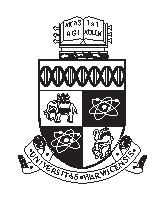
\includegraphics[width=0.4\textwidth]{crest.eps}
	\end{figure}
	\vspace{37mm}
	Cem Yilmaz \\
	\today
	\end{center}
	\end{titlepage}	
	\newpage
	\tableofcontents
	\newpage
\section{Analysis of Algorithms}
\subsection{Classification of a good algorithm}
A good algorithm is one that optimises the following:
\begin{itemize}
	\item Time
	\item Memory
	\item Network bandwidth
	\item Energy consumption
\end{itemize}
However, the main focus in this module will be the running time, in particular, this $O(x)$
\subsection{Running Time}
Running time of an algorithm typical grows with the input size. However, for different inputs of the same size the running time of an algorithm can vary. Then, for an input of fixed size $n$, we have different running times. We can categorise them as the following:
\begin{itemize}
	\item Average case - the typical running time an algorithm requires and is often very difficult to determine
	\item Best case - what is the minimum running time of the algorithm and is generally not useful
	\item Worst case - upper bound on the running time, for any possible input and is more standard to analyse. Our focus is generally this.
\end{itemize}
\subsection{Finding the running time}
\subsubsection{Experimental Analysis}
The first method to use is experimental analysis. For this, we use computer and run simulations. For this, we write a program implementing the algorithm and run the program with inputs of varying size and composition, noting the time needed. However, there are limitations:
\begin{itemize}
	\item It is necessary to implement the algorithm. Sometimes this can be impossible.
	\item Need to make sure that we have considered all kinds of inputs. This sometimes cannot be possible and otherwise it would not be indicative of running time
	\item Different algorithms may run different in different systems due to different features. It can be especially worse for different hardware.
\end{itemize}
\subsubsection{Theoretical Analysis}
The second method is theoretical analysis. For this, we use pen and paper. We use a high-level description of the algorithm instead of an implementation. We then characterise running time as a function of the input size $n$ which takes in account all possible inputs. This would indeed allow us to evaluate the speed of an algorithm independent of the hardware or software environment. A good way to do high level description is to use pseudo-code. We also assume that the algorithm runs in an idealised machine. We assume simple memory hierarchy that is unbounded, infinite precision in arithmetic operations etc. 
\subsection{Random Access Machine (RAM) Model}
It is a simple mode of computation with a singular CPU. It only executes a single program. It also has a bank of memory cells where each cell can hold arbitrarily large positive integers. Every cell gets assigned an ID that allows us to access the information in some \textit{unit time}. In CPU, as learned from CS132, the CPU has the program stored inside. It is also connected to a program counter and registers $R_0,R_1,\ldots$ along with memory cells. It can do basic operations between two numbers stored in the registers, which include but are not limited to:
\begin{itemize}
	\item Addition
	\item Comparison
	\item Fetch an element from the memory
	\item Write an element to the memory
\end{itemize}
However, one thing that categorises and defines RAM as what it is is the fact that \textit{we can access any memory cell in unit times}. 
\subsection{Primitive Operations}
Primitive operations are basic computations that are performed by an algorithm. These take constant time in the RAM model and we count the primitive operations that happen. The assumption is that the number of primitive operations are proportional to the actual running time. Some examples of primitive operations include evaluating an expression, assigning a value, calling a method, indexing into an array etc.
\begin{tcolorbox}[colback=black!3!white,colframe=black!60!white,title=\begin{exmp}Operations in a code \label{Operations in a code}\end{exmp}]
        \begin{lstlisting}[language = Java , caption={Operations} , frame = trBL , firstnumber = last , escapeinside={(*@}{@*)}]
        public static double arrayMax(double[] data) {
		int n = data.length;
		double currentMax = data[0];
		for (int j = 1; j < n; j++)
			if (data[j] > currentMax)
				currentMax=data[j];
		return currentMax;
	}
        \end{lstlisting}
	In particular,
	\begin{itemize}
		\item Step $3$ has $2$ operations
		\item Step $4$ has $2$ operations
		\item Step $5$ has $2n$ operations
		\item Step $6$ has $2n-2$ operations
		\item Step $7$ has $2n-2$ operations and finally
		\item Step $8$ has $1$ operation.
	\end{itemize}
	The code for $arrayMax$ has $6n+1$ as the worst case and $4n+3$ as the best case. Let $T(n)$ be the running time of arrayMax. Then, 
	\begin{align*}
		a(4n+3) \le T(n) \le a(6n+1)
	\end{align*}
Where $a$ is the time to execute a primitive operation.
\end{tcolorbox}
\subsection{Sorting algorithms}
Indeed, the time complexity can be seen clearly in sorting algorithms for times.
\begin{figure}[H]
	\centering
	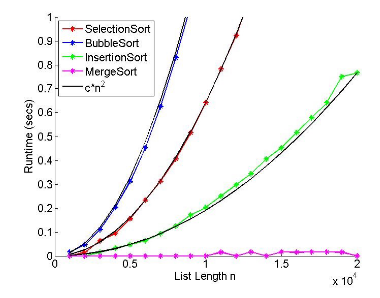
\includegraphics[width=0.6\textwidth]{sorting.png}
	\caption{Complexity of sorting algorithms}
	\label{fig:sorting-png}
\end{figure}
\section{Asymptotic Notation}
\subsection{Big-O notation}
\begin{tcolorbox}[colback=black!3!white,colframe=black!60!white,title=\begin{defn}Big O \label{Big O}\end{defn}]
For two functions $f(n)$ and $g(n)$, we say that $f(n)$ is $O(g(n))$ if there are positive constants $c$ and $n_0$ i.e. $n_0,c\ge 1$ and such that
\begin{align}
	f(n) \le cg(n)
\end{align}
for any $n \ge n_0$ and $n \ge n_0$.
\end{tcolorbox}
\begin{tcolorbox}[colback=black!3!white,colframe=black!60!white,title=\begin{exmp}Example 1 \label{Example 1}\end{exmp}]
        $2n+10$ is in $O(n)$.
                \begin{align}
                2n+10 \le  cn \\
		(c-2)n \ge 10 \\
		n\ge \frac{10}{c-2}
                \end{align}
		We pick $c=3$ and $n_0=10$.
\end{tcolorbox}
\begin{tcolorbox}[colback=black!3!white,colframe=black!60!white,title=\begin{exmp}Example 2 \label{Example 2}\end{exmp}]
        $n^2$ is not $O(n)$
                \begin{align}
                n^2\le cn\\
		n\le c
                \end{align}
		$c$ is a constant and thus this inequality cannot be satisfied.
\end{tcolorbox}
\begin{tcolorbox}[colback=black!3!white,colframe=black!60!white,title=\begin{exmp}Example 3 \label{Example 3}\end{exmp}]
        $7n-2$ is in $O(n)$
                \begin{align}
                7n-2 \le cn
                \end{align}
		Pick $c=7$ and $n_0=1$.
\end{tcolorbox}
\begin{tcolorbox}[colback=black!3!white,colframe=black!60!white,title=\begin{exmp}Example 4 \label{Example 4}\end{exmp}]
        Is is true that $t>0$, $(1+n) ^{t}$ is in $O(n^{t})$
                \begin{align}
			(1+n)^{t} = \sum_{i=0}^{t} {t \choose i} n^{i}
                \end{align}
		However, $t$ is the biggest number therefore it is $O(n^{t})$
\end{tcolorbox}
Thus, the Big-O notation gives an upper bound on the growth rate of a function as $n$ grows towards infinity. We can use the Big-O notation to rank functions according to their growth rate.
\subsubsection{General Rules}
\begin{itemize}
	\item Drop lower order terms
	\item Drop constant terms
	\item Use the smallest possible class of functions
\end{itemize}
\section{Relatives of Big-O}
\subsection{Big Omega}
\begin{tcolorbox}[colback=black!3!white,colframe=black!60!white,title=\begin{defn}Big Omega \label{Big Omega}\end{defn}]
$f( n)$ is $\Omega(g(n))$ if there is a constant $c > 0$ and an integer constant $c>0$ and an integer constant $n_0\ge 1$ such that for $n\ge n_0$
\begin{align}
f(n) \ge cg(n)
\end{align}
\end{tcolorbox}
\subsection{Big Theta}
\begin{tcolorbox}[colback=black!3!white,colframe=black!60!white,title=\begin{defn}Big Theta \label{Big Theta}\end{defn}]
$f(n)$ is $\Theta(g(n))$ if there are constants $c'>0$ and $c'' > 0$ and ann integer constant $n_0 \ge 1$ such that for $n \ge  n_0$
\begin{align}
c'g(n) <f(n) \le c''g(n)
\end{align}

\end{tcolorbox}
\subsection{Summary}
\begin{itemize}
	\item Big-$O$ is asymptotically less than or equal to $g(n)$ 
	\item Big-$\Omega$ is asymptotically greater than or equal to $g(n)$ 
	\item Big-$\Theta$ is asymptotically sandwiched between $g(n)$ differing by constant
\end{itemize}
\begin{figure}[H]
    \centering
    \incfig{summaryo}
    \caption{Summary of Big notations graphically}
    \label{fig:summaryo}
\end{figure}
\subsection{Examples}
\begin{tcolorbox}[colback=black!3!white,colframe=black!60!white,title=\begin{exmp}Example 1 \label{Example 1}\end{exmp}]
        $5n^2$ is in $\Omega(n^2)$
                \begin{align}
                5n^2\ge cn^2, \text{ let } c=5, n_0=1
                \end{align}
	$5n^2$ is also $\Omega(n)$
	\begin{align}
		5n^2\ge cn, \text{ let }c=1, n_0=1
	\end{align}
	$5n^2$ is in $O(n^2)$
	\begin{align}
		5n^2 < cn^2, \text{ let } c=6, n_0=1
	\end{align}
	Because $\Omega(n^2)$ and $O(n^2)$, we indeed can say that
	\begin{align}
		\Theta(n^2)
	\end{align} 
\end{tcolorbox}
\section{Data Structures}
\subsection{Arrays}
\begin{tcolorbox}[colback=black!3!white,colframe=black!60!white,title=\begin{defn}Array \label{Array}\end{defn}]
An array is a sequences collection of variables of thesame type. Each variable, or cell, in an array has an index, which uniquely refers to the value stored in that cell.

A value stored in an array is often called an element.

The length of an array determines the maximum number of elements that can be stored.
\end{tcolorbox}
\subsubsection{Strengths}
\begin{itemize}
	\item We assume that we can access each cell $k$ in $O(1)$ time.
	\item You can write or read once accessed.
	\item Access time is very fast $O(1)$.
\end{itemize}
\subsubsection{Limitations}
\begin{itemize}
	\item We cannot change the length of an array
\end{itemize}
\subsubsection{Declaring arrays in Java}
Assignment to a literal form when initially declaring the array
\begin{lstlisting}[language = Java , caption={Array} , frame = trBL , firstnumber = last , escapeinside={(*@}{@*)}]
elementType[] arrayName = { v0, v1, ..., vn-1}
\end{lstlisting}
elementType : any Java base type, or class name

arrayName : any valid Java identifier

Remark : the initial values must be of the same type as the array.

We also use the new operator to declare arrays because it is not an instance of a class. That is,
\begin{lstlisting}[language = Java , caption={Declaring array} , frame = trBL , firstnumber = last , escapeinside={(*@}{@*)}]
new elementType[length]
\end{lstlisting}
The new operator returns a reference to the new array. This is assigned to the array variable measurements.
\begin{lstlisting}[language = Java , caption={Example} , frame = trBL , firstnumber = last , escapeinside={(*@}{@*)}]
double [] measurements = new double [1000]
\end{lstlisting}
\subsubsection{Examples}
A array can store primitive elements, such as characters. E.g.
\begin{table}[H]
	\centering
	\caption{Primitive element array}
	\label{tab:label}
	\begin{tabular}{|c|c|c|c|c|c|}
	\hline
	S & A  & M  & P  & L & E  \\
	\hline
	0 & 1 & 2 & 3 & 4 & 5 \\
	\hline
	\end{tabular}
\end{table}
...or pointer to references to objects. For example, the first cell can refer to the pointer of the word "Joseph" and the second can refer to the pointer of "Helen" etc.
\subsubsection{Adding an entry}
To add an entry $e$ into array board at $i$ we need to make room. We shift each $n-i \mapsto n-i+1$. This is $O(n-i)$.
\subsubsection{Concluding Remarks}
\begin{itemize}
	\item Read/write any element in $O(1)$ time
	\item The capacity does not change
	\item Shifting $k$ elements requires $O(k)$ time
	\item Very easy to work with
	\item We are going to use arrays a lot when we implement
\end{itemize}
\subsection{Linked Lists}
\subsubsection{Singly Linked List}
\begin{tcolorbox}[colback=black!3!white,colframe=black!60!white,title=\begin{defn}Singly Linked List \label{Singly Linked List}\end{defn}]
A singly linked list is a conrete data of structure consisting fro a sequence of nodes, starting from a head pointer.
\end{tcolorbox}
Each node stores element and a link to the next node. However, nodes do not have information on previous nodes. The first node is usually called head, and the last is called tail. However, if the node is tail, then the next link is NULL. However, to access $k$-th element in the node, we would then require to repeat getting node $k-1$ times. This is called pointer hopping.
\subsubsection{Time required for Singly Linked List}
Our assumption is that CurrentNode.getNext() requires $O(1)$ time. In order to access $k$-th element, we need $O(k)$ time.
\subsubsection{Insertion - Operations}
To insert a head:
\begin{itemize}
	\item Allocate a new node
	\item Insert a new element
	\item New node points to old head
	\item Update head to point new node
\end{itemize}
\end{document}





